\documentclass[11pt,a4paper]{article}
\usepackage{amsmath}
\usepackage[utf8]{inputenc}
\usepackage{graphicx}	%Grafiken


\title{Abstract of Computer Graphics}
\author{Andreas Ruscheinski \ Christian Delfs}
\date{}
\begin{document}
\maketitle

\section{Introduction}
	\subsection{What is Computer Graphics?}
		\begin{itemize}
			\item deals with all aspect of image creation with computers
		\end{itemize}
	\subsection{Application Areas}
	\subsection{History}
	\subsection{Image formation}
		\begin{itemize}
			\item form images on a two dimensional device analogous how images are formed by physical systems (Cameras and so on)
			\item Objects, Viewer, Light sources with attributes how light interacts with materials in scene, IMPORTEND: independence of object, viewer and light sources
			\item Ray Tracing: follow rays from light with maybe collusions with object to lens (camera) or going to infinity
			\item Luminance Image: Monochromatic (grey levels) like black-white-films
			\item Color Image: perceptional attributes (hue, saturation, lightness)
			\item Additive Color: adding amouts of three primaries (RGB), Monitor
			\item Subtractive Color: form color by filter white light (CYM), Printing
			\item Pinhole Camera: use trigonometry to find project 
			\begin{center}
				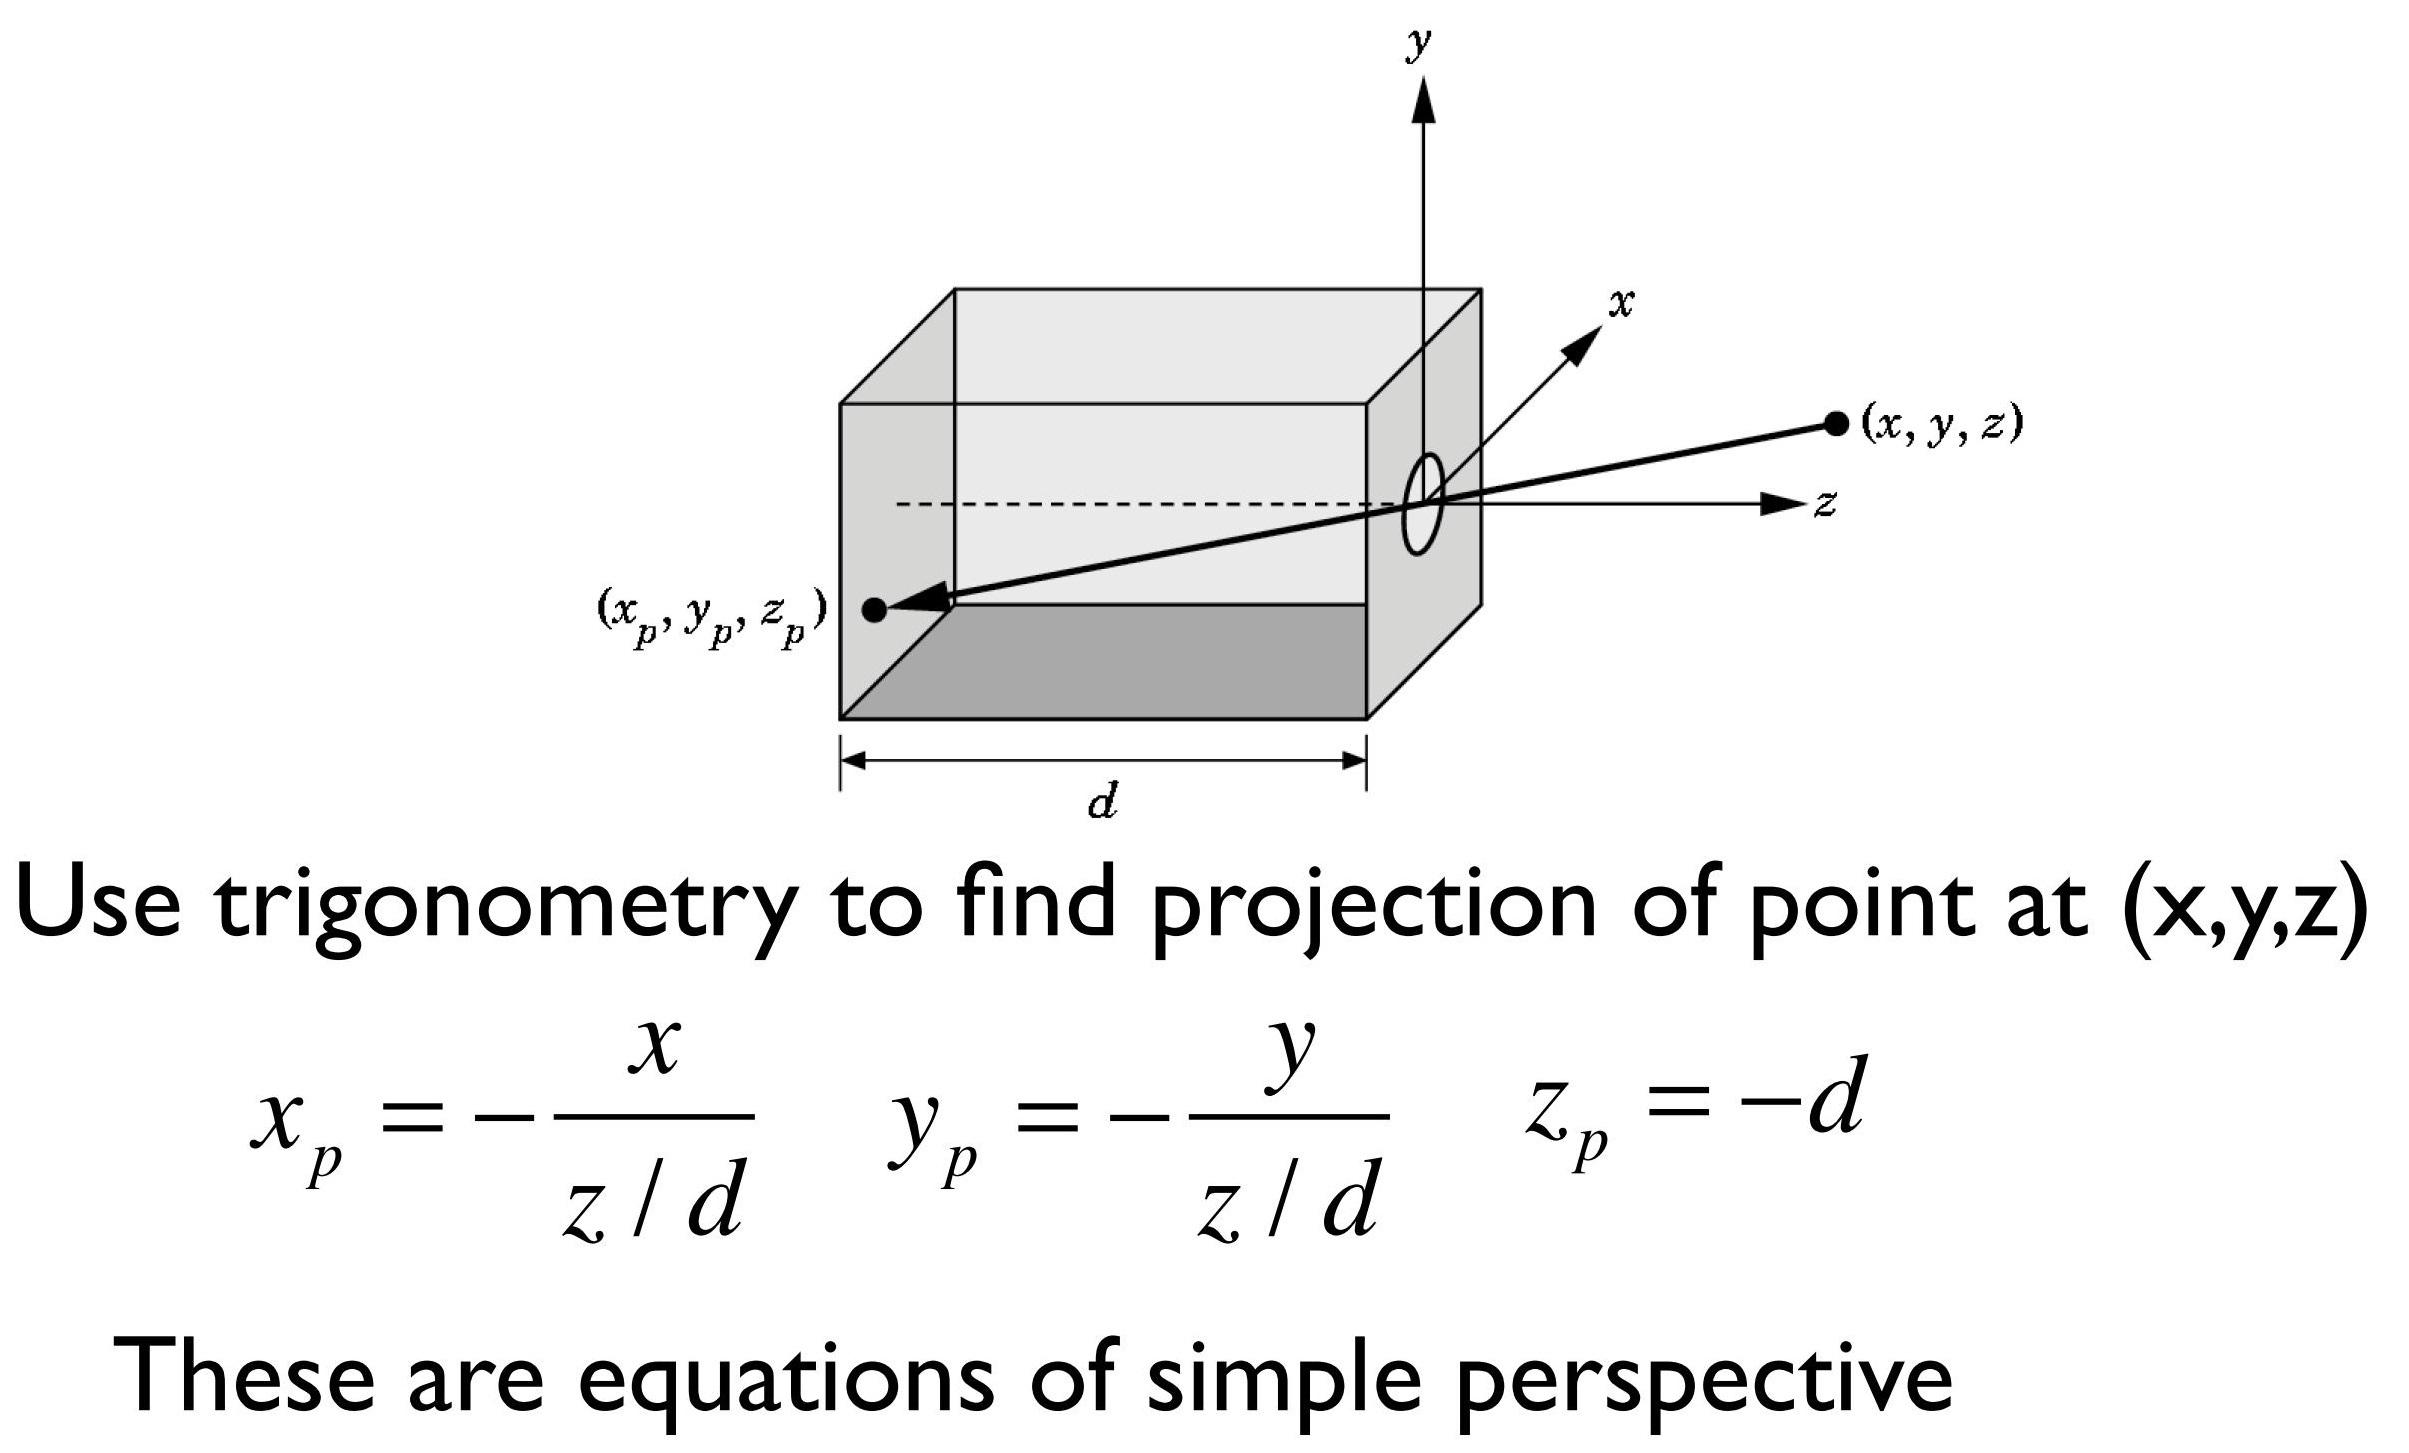
\includegraphics[scale=0.3]{pictures/pic1.jpg}
			\end{center}
			\item Synthetic Camera: projection of image on image plane, camera views on image plane ?????
			\item Advantages of SC: separation of objects, viewer, light sources, two-dimensional graphics is a special case of three-dimensional graphics, simple api with fast hardware implementation
			\item cant compute color or shade of each object independently reasons: blocked form light, reflects, translucent
			\item disadvantages of ray tracing: easy calculation for easy object, but on compley objects FUCK UP especially with lights and shadows
		\end{itemize}
	\subsection{Basic Architecture} 
		\begin{itemize}
			\item Physical Approaches: RayTracing = SLOW, can handle global effects; Radiosity: Energy based approaced = MUCH SLOWER
			\item Practical Approaches: process one object at time, can only handle local lightning, pipeline architecture
			\begin{center}
				
\includegraphics[scale=0.5]{pictures/pic4.jpg}
			\end{center}
			\item Vertex Processing: much work is converting object representations form one coordinate system to another (Object Coordinates, Camera Coordinates, Screen Coordinates)
			\begin{itemize}
				\item Projection: combines 3D viewer with the 3D objects to produce the 2D image
				\item Perspective Projection: all Projectors meet the center of projection
				\item Parallel Projection: projectors are parallel, center of projection is replaced by a direction of projection
			\end{itemize}
			\item Primitve Assembly: vertices must be collected into geometric objects (line segments, polygons, curves and surfaces)
			\begin{itemize}
				\item Clipping: a real camera cannot see the whole world, objects that are not within this volume are said to be clipped out of the scene
			\end{itemize}
			\item Rasterization: create fragments (potential pixels), fragments have locations in frame buffer, color and depth attributes, vertex attributes are interpolated over objects by the rasterizer
			\item Fragment Processing: fragments are processed to determinate the color of pixel in frame buffer, color determined by texture mapping or interpolation of vertex colors, fragments may blocked by other fragments coloser to camera (hidden surface removal)
			\item Programmiers Interface:
			\begin{itemize}
				\item API
				\item specifiy what we nee to form an image (objects, viewer, light sources, materials), handling input from devices
				\item Object Specification: limited set of primitives (points, line segments, polygons, some surfaces)
				\item Camera Specification: postion of center of lens, orientations, lens, film size, orientation of film plane
				\item Light: different types of lights (point lights, spot light, near and far sources, color properties)
				\item Material: absorption, diffuse, specular
			\end{itemize}
		\end{itemize}
	\subsection{RayTracing}
		\begin{itemize}
			\item follow rays of light from a point source
			\item Problems: rays do not affect what we see, scattering produces many rays; Better: ray casting
			\item Ray Casting: rays goes from view to scene, one ray for one pixel
			\item objects are build from primitives and set operations with other objects
			\item Ray is parametric, Sphere is quadric (quadric is a solution set of quadratic functions), Resulting equations is a entry/exit point or no solution if ray misses
			\item one point is visable if we hit light source form point
			\item in case of reflection follow rays from transmitting surfaces, recursive process
			\item Structure: recursivly, calculate for each ray, find intersection with closet surfaces (need object datebase, complexity of calculation limits of object types), compute lightnig at surface, trace reflected and transmittet rays
			\item stop of procedure if no track amout left (some light will be absorbed at each intersetion with object), ignore rays that go of to infinity (workaround, large absorbing sphere around problem), cout steps
			\item color of pixel is the result of local+reflected+transmitted
			\item Computing Intersections, solve equations with maybe nurmerical methods 
			\item easy calculation with planes
			\item polyhedra build from planes
			\item ray enters at furthest intersection with front facing plane, leaves at closest intersection with back facing planes,
			\item if entry is further away then exit,ray muss miss the polehedron
		\end{itemize}

\section{Basic OpenGL}
	\subsection{Architecture}
		\begin{itemize}
			\item  a platform-independent API (Easy to use,  Close enough to the hardware to get excellent performance)
			\item  Focus on rendering
			\item Relatively stable
			\item Evolution reflect new hardware capabilities (3D texture mapping and texture objects, Vertex programs)
			\item OpenGL Libraries
				\begin{itemize}
					\item OpenGL core library (OpenGL32 - Windows,  GL - most unix/linux systems (libGL.a))
					\item OpenGL Utility Library (GLU) (Provides functionality in OpenGL core but avoids having to rewrite code)
				\end{itemize}
			\item OpenGL Functions
				\begin{itemize}
					\item Primitives (Points, Line Segments, Polygons)
					\item Attributes
					\item Transformations (Viewing, Modeling)
					\item Control (GLUT)
					\item  Input (GLUT)
					\item Query
				\end{itemize}
			\item OpenGL Architecture
			\begin{center}
				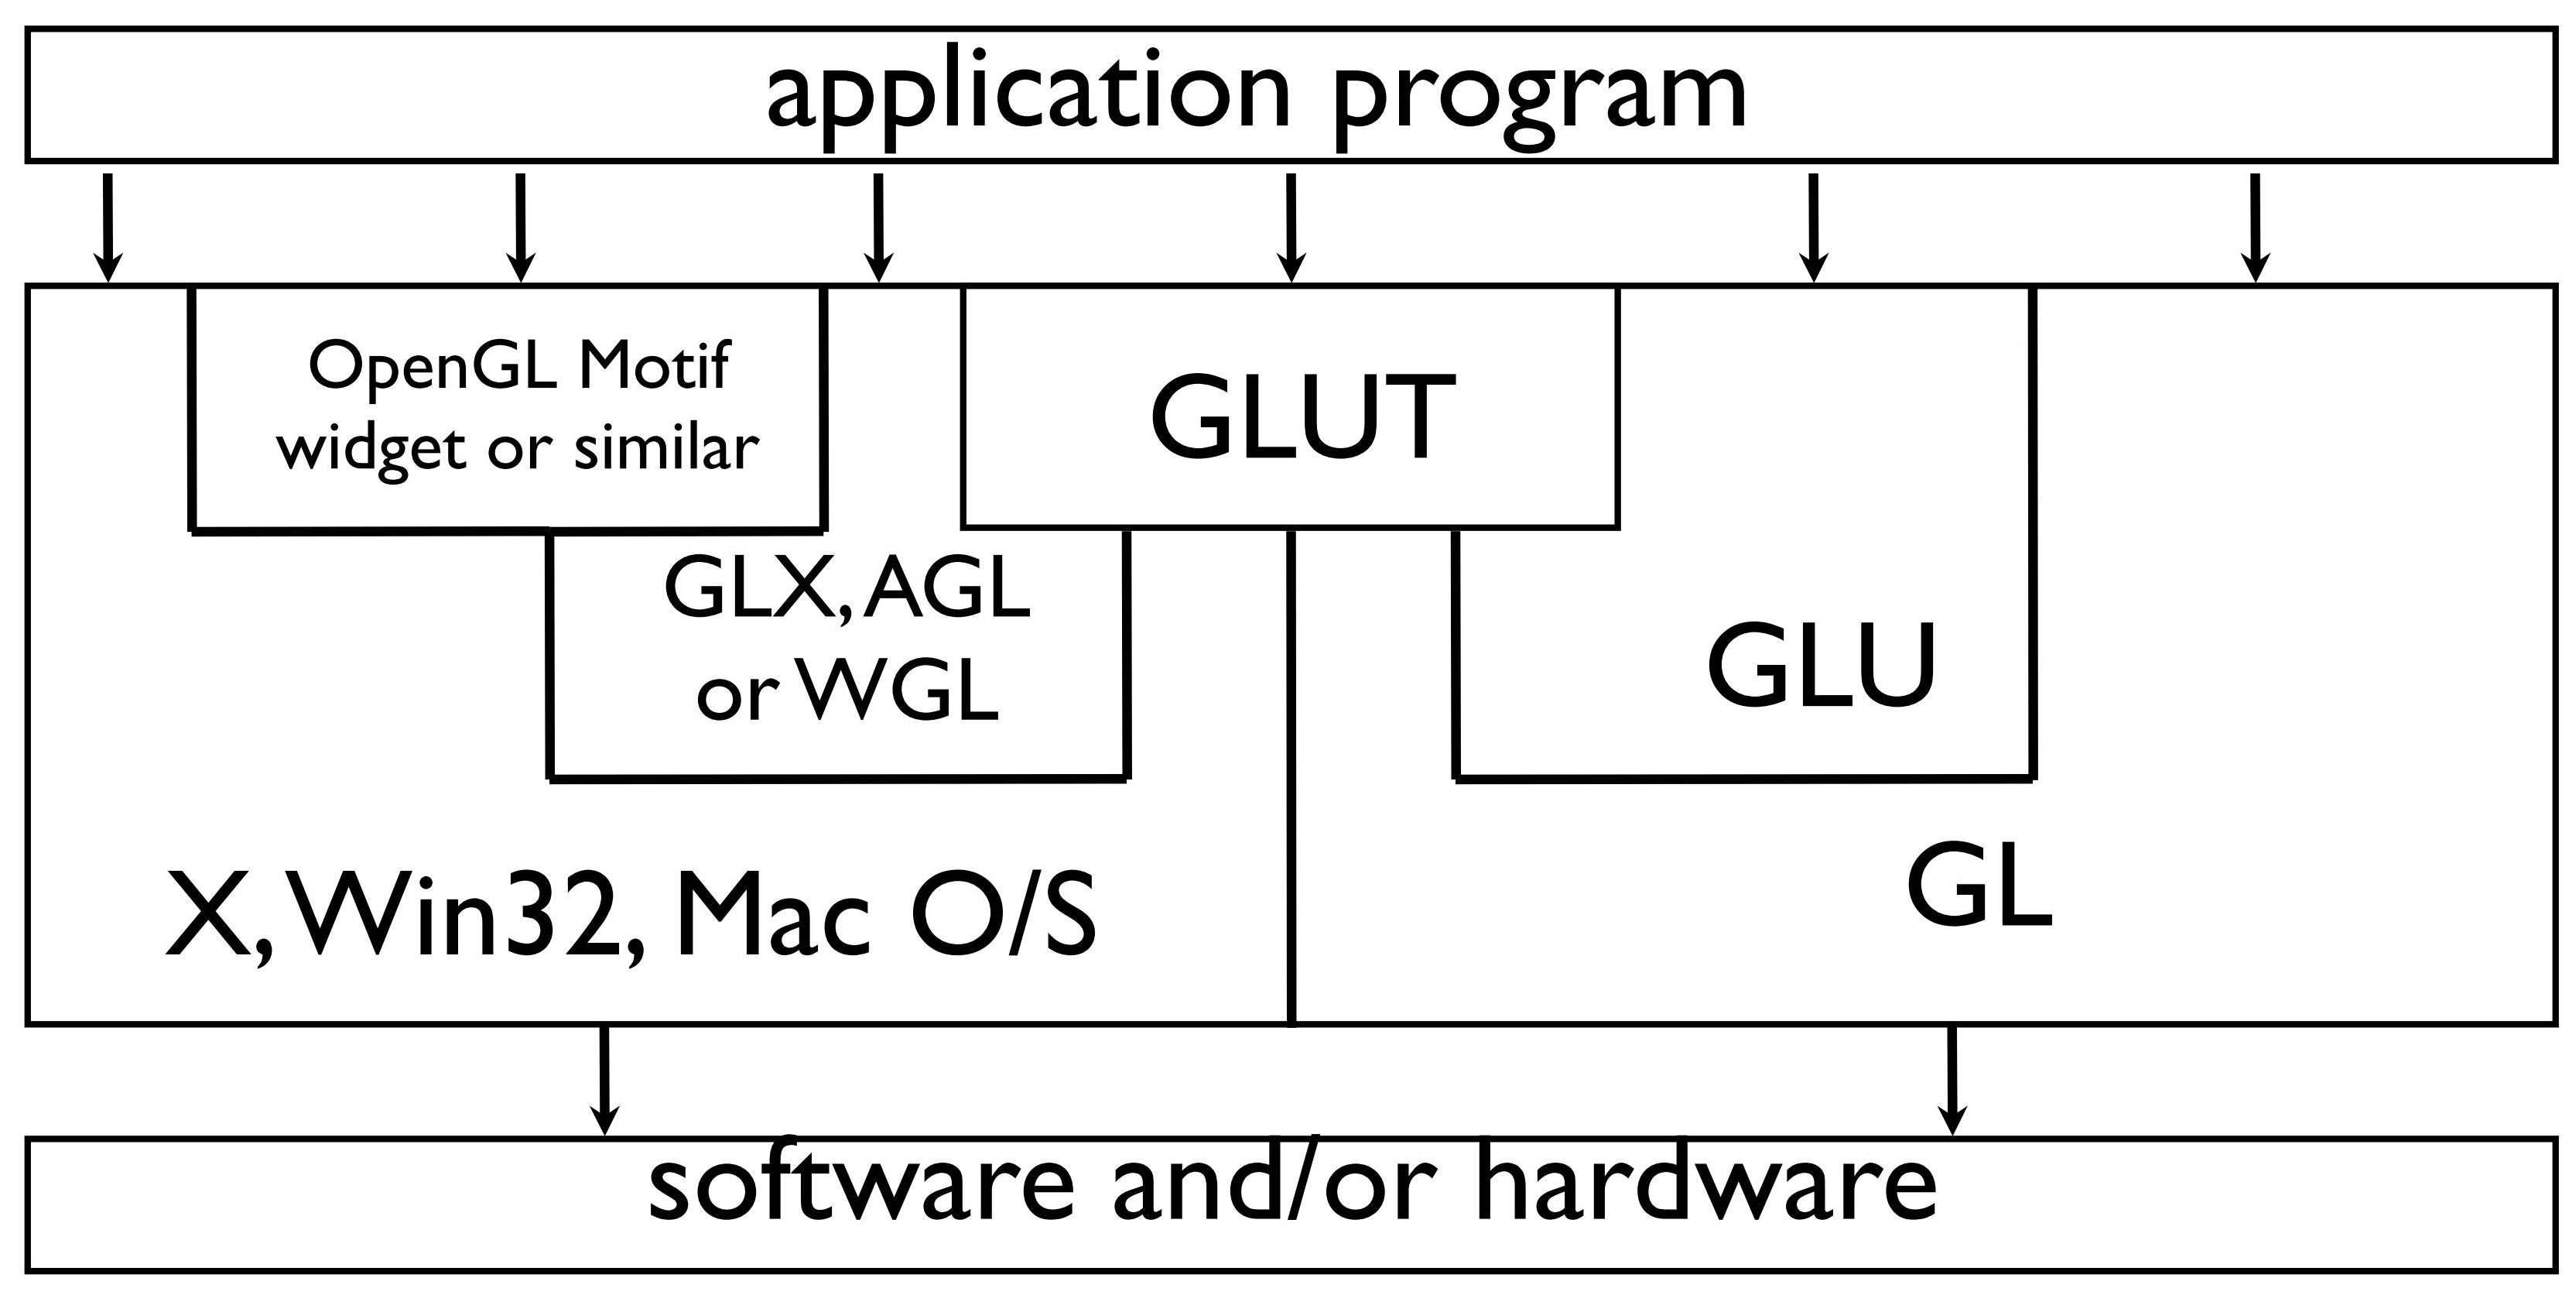
\includegraphics[scale=0.3]{pictures/pic2.jpg}
			\end{center}
			\item Software Organization
			\begin{center}
				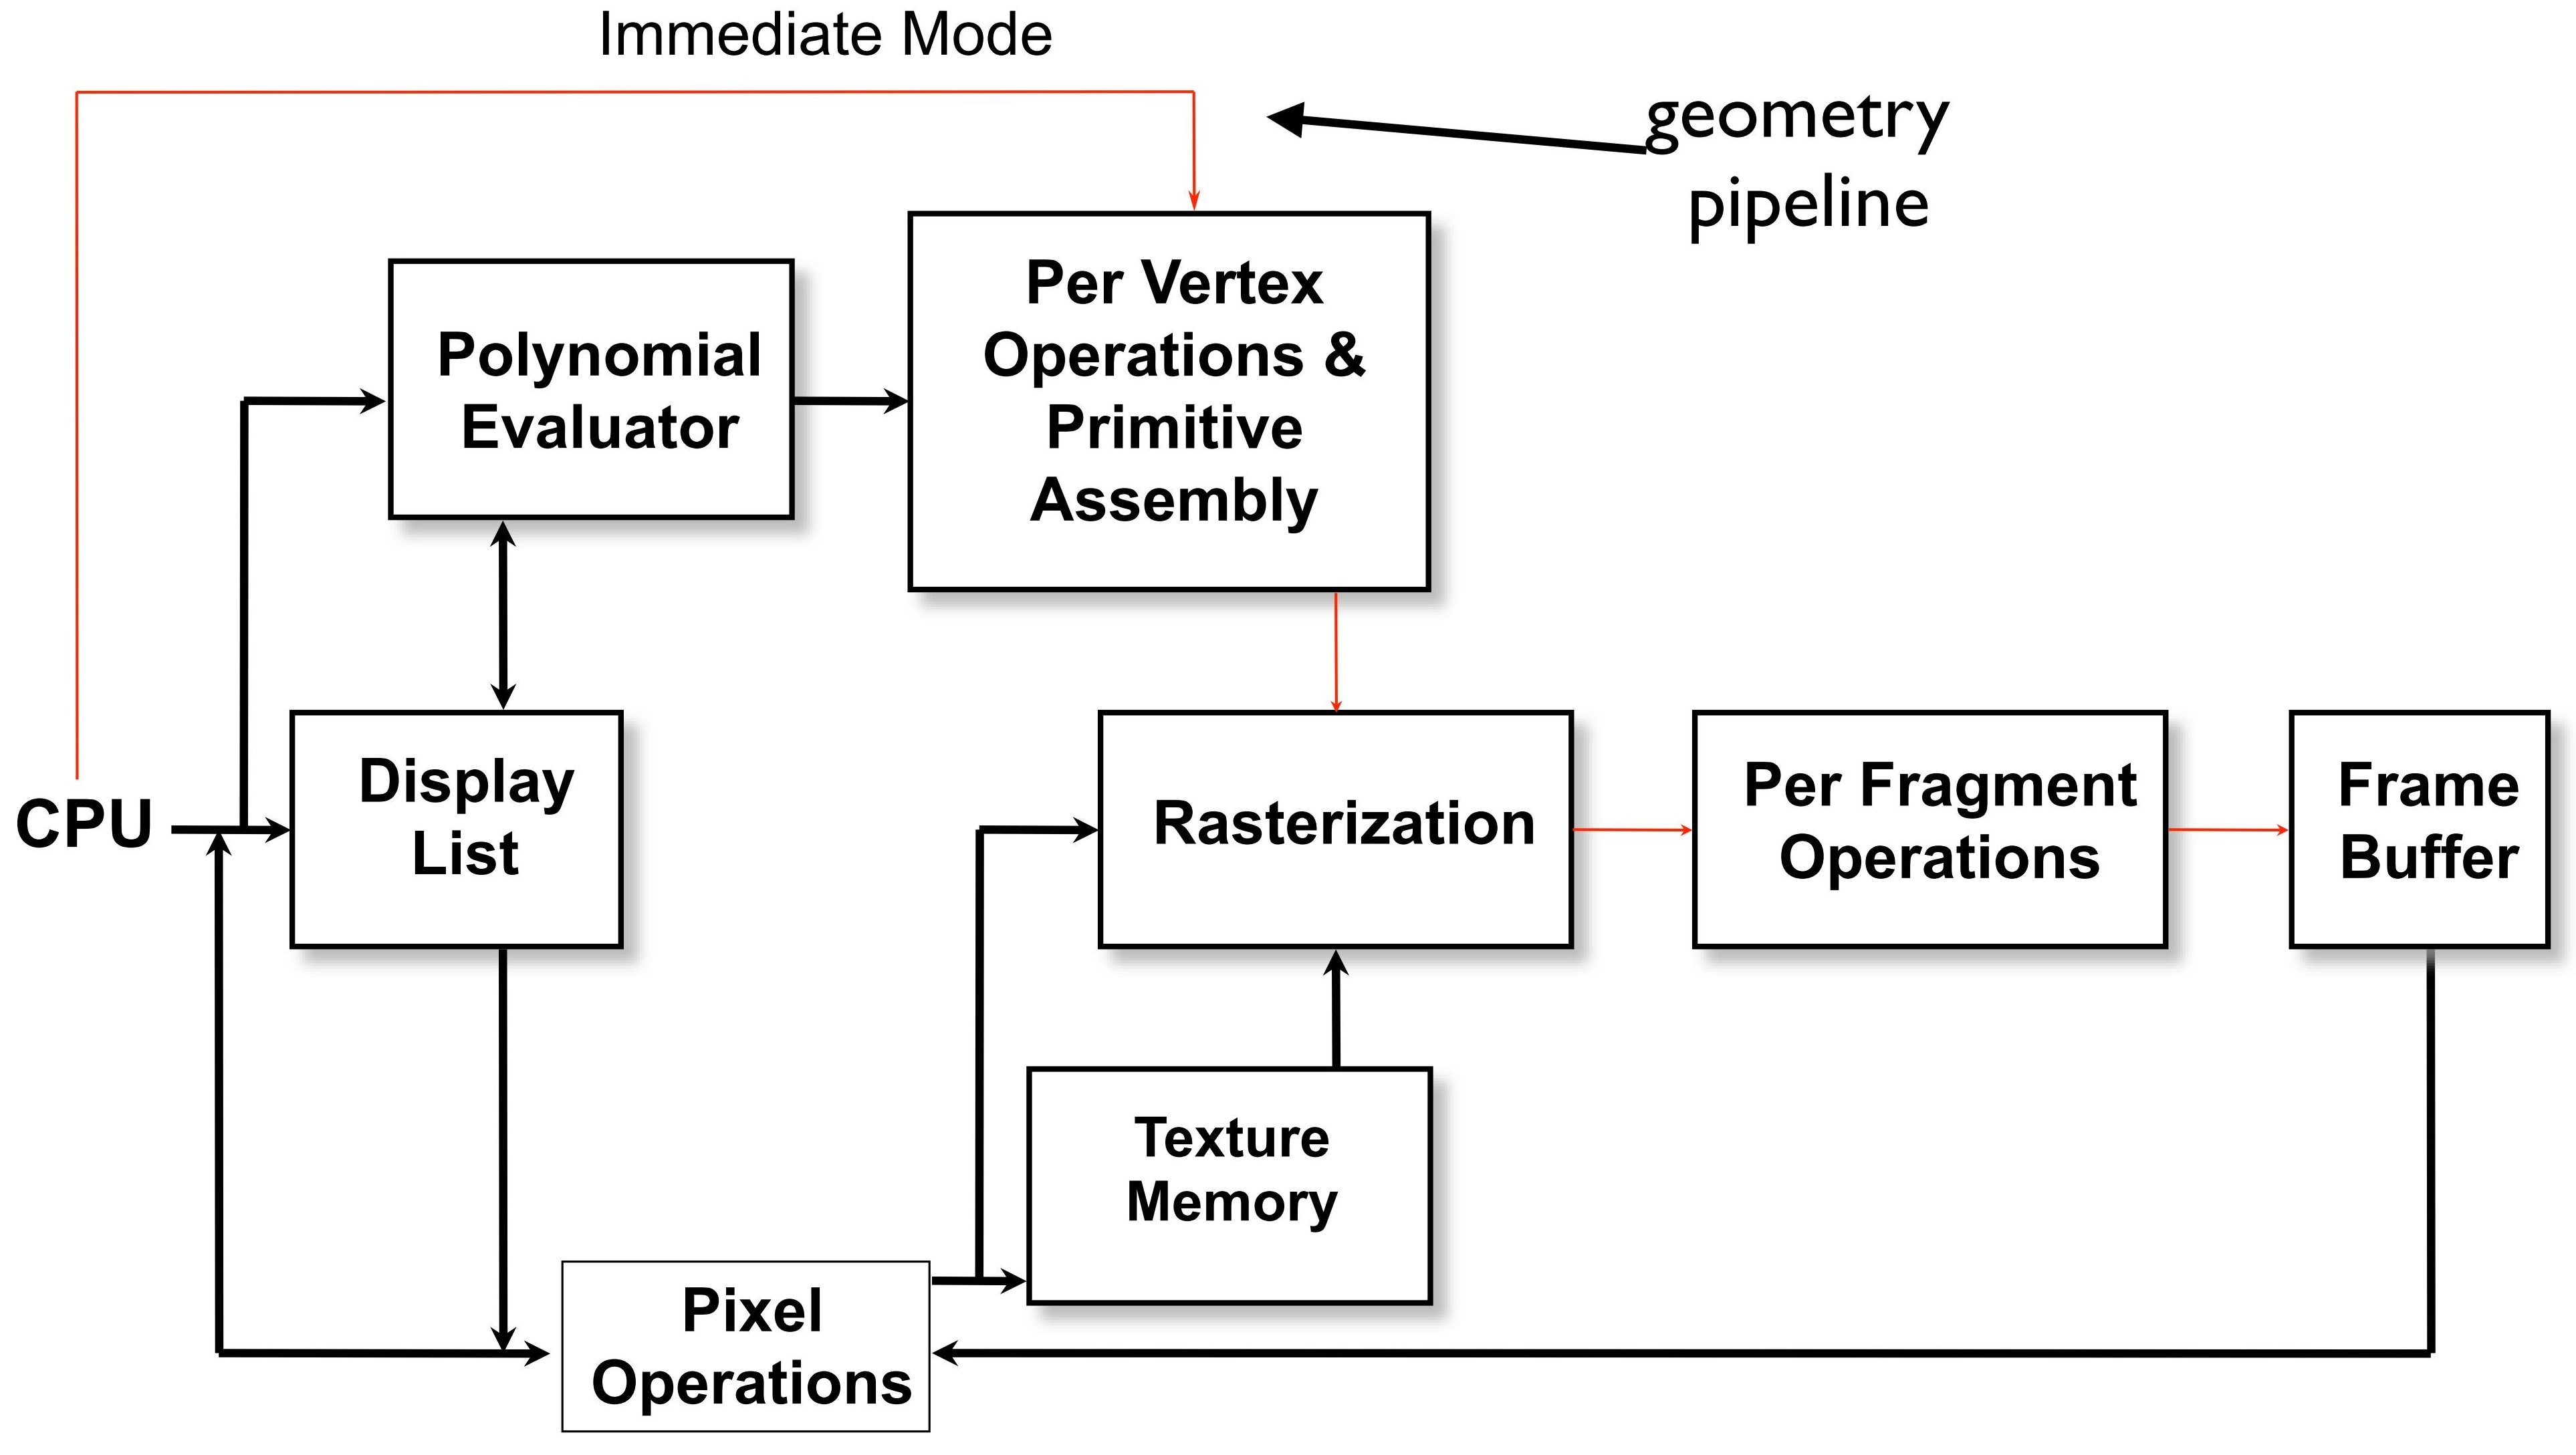
\includegraphics[scale=0.3]{pictures/pic3.jpg}
			\end{center}
			\item OpenGL is a state machine
			\item OpenGL functions are of two types
				\begin{enumerate}
					\item Primitive generating \\
						(Can cause output if primitive is visible, How vertices are processed and appearance of primitive are controlled by the state)
					\item State changing\\
						(Transformation functions, Attribute functions)
				\end{enumerate}
			\item OpenGL is not object oriented so that there are multiple functions for a given logical function (glVertex3f, glVertex2i, glVertex3dv)
		\end{itemize}
	\subsection{GLUT - OpenGL Utility Toolkit}
		\begin{itemize}
			\item  Provides functionality (Open a window, Get input from mouse and keyboard, Menus, Event-driven)
		\end{itemize}
	\subsection{Simple programs in two and three dimensions}
		\begin{itemize}
			\item  Event Loop
			\begin{itemize}
				\item Note that the program defines a display callback function named mydisplay
				\item Every glut program must have a display callback
				\item The display callback is executed whenever OpenGL decides the display must be refreshed, for example when the window is opened
				\item The main function ends with the program entering an event loop
			\end{itemize}
		\end{itemize}
	\subsection{Interaction}
		
\section{Three-Dimensional Graphics}
	\subsection{Geometry}
	\subsection{Representation}
	\begin{itemize}
		\item Lineare Independance: a set of vectors are linearly independent $\leftrightarrow \alpha_{1}v_{1}+\alpha_{2}v_{2}+\alpha_{3}v_{3} +\dots = 0$ iff $\alpha_{1}=\alpha_{2}=\alpha_{3}\dots = 0$ thats mean that no vector can be written in combination with the others
		\item Dimension: in vector space the maximum number of l. independent vectors is fixed and is called the dimension, in an n-dimensional space any set of n linearly independent vectors form a basis, any vector v can be written in combination with basis $v_{1},v_{2},v_{3},\dots,v_{n}$ and $v= \alpha_{1}v_{1}+\alpha_{2}v_{2}+\alpha_{3}v_{3} +\dots+\alpha_{n}v_{n}$ where $\{\alpha_{i}\}$ is unique
	\end{itemize}
	\subsection{Transformations}
	\subsection{Homogeneous Coordinates}
	\subsection{Viewing}
	\subsection{Shading}

\section{Implementation}
	\subsection{Approaches (object vs image space)}
	\subsection{Implementing the pipeline}
	\subsection{Clipping}
	\subsection{Polygon Fill}
	
\section{Discrete Methods}
	\subsection{Buffers}
	\subsection{Bitmaps and Pixel Maps}
	\subsection{Texture Mapping}

\section{Programmmable Pipelines}
	\subsection{Shading Languages}
	\subsection{GLSL}
	\subsection{Vertex Shaders}
	\subsection{Fragment Shaders}

\section{Curves and Surfaces}
	\subsection{Representation of Curves and Surfaces}
	\subsection{Bézier Curves and Surfaces}
	\subsection{B-Splines}

\section{Advanced Rendering}
	\subsection{Radiosity}

\section{Hierarchies and Parallel Rendering}7
	 \subsection{Traversal Methods}
	 \subsection{Scene Graphs}
	 \subsection{Parallel Rendering}

\end{document}

	